\documentclass{article}
\usepackage{hyperref}
\usepackage[procnames]{listings}
\usepackage{color}
\title{Assignment 5}
\date{2016-03-03}
\author{Tarek Fouda}
\usepackage[pdftex]{graphicx}
\usepackage{listings}
\usepackage{alltt}

\definecolor{dkgreen}{rgb}{0,0.6,0}
\definecolor{gray}{rgb}{0.5,0.5,0.5}
\definecolor{mauve}{rgb}{0.58,0,0.82}

\lstset{
	basicstyle=\footnotesize,
	breaklines=true,
}

\begin{document}
  \maketitle


\section{Problem 1} \label{problem1}

\subsection{What is Karate club graph?}

Basically, there was a karate club that consists of 34 individual. The Karate club was observed for a period of three years. At the beginning of the study, the club president, John A., and Mr. Hi argued over the price of the Karate lessons. The president wished to stabiliz the prices while the instructor, Mr. Hi, wished to raise prices. By the time, the whole club split into two parts, one who agrees with the instructor and the other who was pro the president. The Graph shows thefriendship ties between all the members (nodes) until the club was divided into two parts.
\begin{figure}
\centering
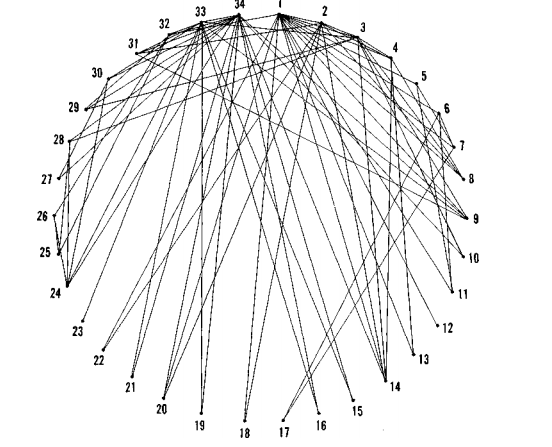
\includegraphics[scale=0.95]{1.png}
\caption{The graphic representation of the social relationships among the 34 individuals in the Karate club}
\label{fig:1.png}
\end{figure}
\newpage

Figure \ref{fig:1.png} represents the relationships among the 34 individuals in the Karate club.The edge in this graph represents the interaction or the friendship between each of the nodes.


Figure \ref{fig:2.png} shows the graph in a more convinient way, where the pink nodes are the nodes that support the instructor, who is node 34, on the other hand, the white nodes are the individuals that support node 1, which is the president.



\begin{figure}
\centering
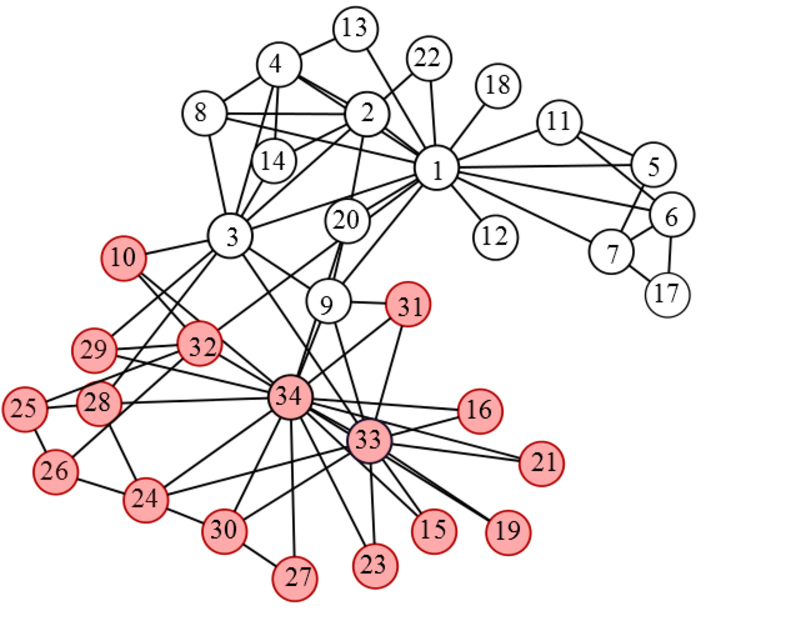
\includegraphics[scale=0.75]{2.png}
\caption{The Karate club}
\label{fig:2.png}
\end{figure}
\newpage
\subsection{Betweeness and grivan newman Algorithm}
The idea of edges betweeness and the Grivan newman algorithm is simple. Initially, if we have a weighted graph we need to calculate the betweeness of all edges and remove the edge with the highest value then recalculate the betweeness  and perform the same steps until the graph is disconnected into two splits.
Keeping in mind that betweeness of the edge is normally the traffic flow in the corresponding edge.
After performing the algorithm on Figure \ref{fig:2.png} and keeping on deleting the nodes with the highest betweeness, we get  Figure \ref{fig:3.png} which proves that it sort of look like the initial Karate club grapghrepresented in Figure \ref{fig:2.png}
\begin{figure}
\centering
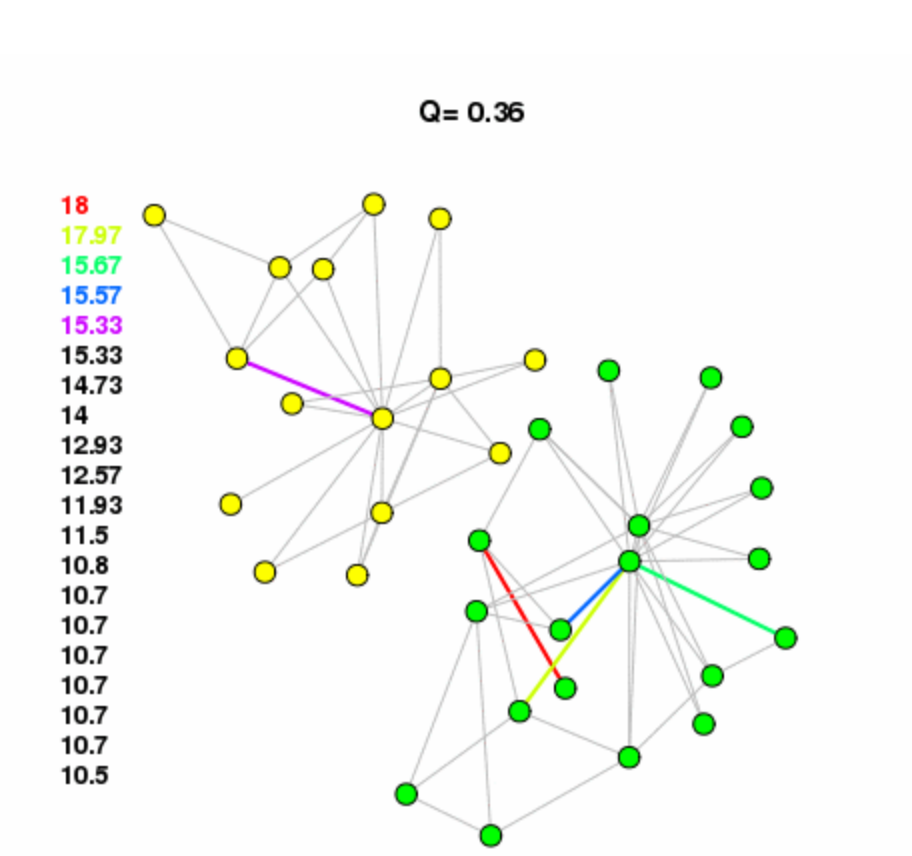
\includegraphics[scale=0.75]{3.png}
\caption{The Karate club after spliiting it into two divisions using grivan newman algorithm}
\label{fig:3.png}
\end{figure}

Moreover if we keep on implementing the algorithm on the graph, it will end up splitting into 3 and 4 groups and so on. 
\begin{figure}
\centering
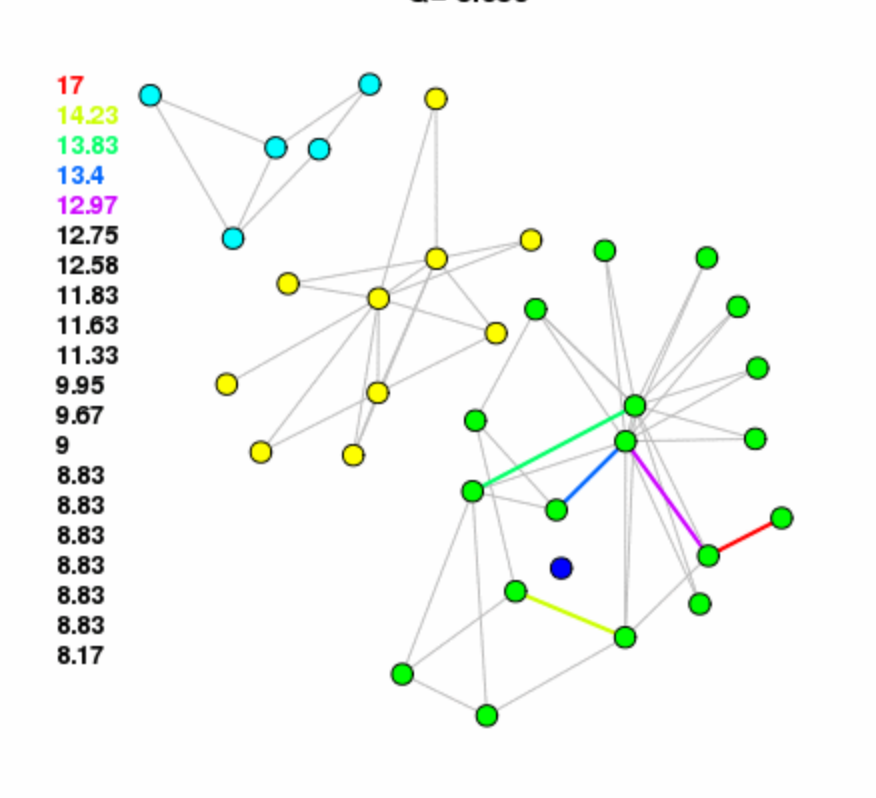
\includegraphics[scale=0.75]{4.png}
\caption{The Karate club after spliiting it into three divisions using grivan newman algorithm}
\label{fig:4.png}
\end{figure}
Figure \ref{fig:4.png} demonstrates that.

\section{References}
The references I used to prove the graphs and to fully understand the concepts were \url{cneurocvs.rmki.kfki.hu/igraph/screenshots2.html} and \url{http://aris.ss.uci.edu/~lin/76.pdf}.
Also grivan newman algorithm was explained well in\url{ http://www-personal.umich.edu/~ladamic/courses/networks/si614w06/ppt/lecture18.ppt}

\url{http://clair.si.umich.edu/si767/papers/Week03/Community/CommunityDetection.pptx}
\end{document}